\section{Implementación}
\label{s3:sec:Implementacion}


\subsection{FPGA}
\label{s3:subsec:fpga}

\todo{Escribir, haciendo referencia a la figura~\ref{s3:fig:componentes-fpga-a}}
\begin{figure}
\todo{No se si esto es muy pequeño y habría que separarlo, o incluso mover
  la imagen de clocking a la sección correspondiente o no}
\centering
\begin{subfigure}{.5\textwidth}
  \centering
  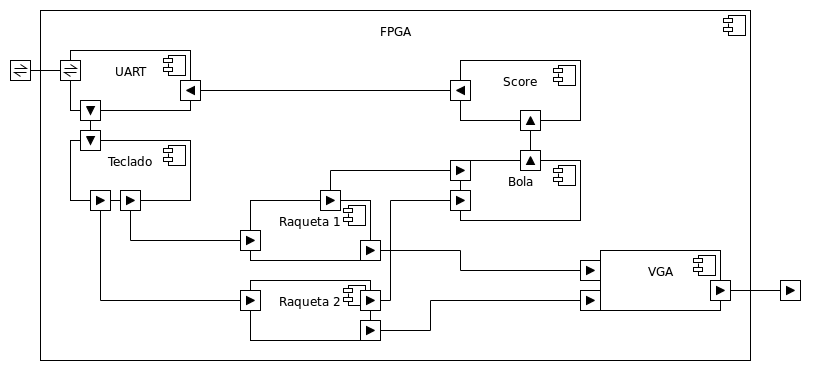
\includegraphics[width=1.0\textwidth]{images/fpga_componentes.png}
  \caption{Componentes implementados.}
  \label{s3:fig:componentes-fpga-a}
\end{subfigure}%
\begin{subfigure}{.5\textwidth}
  \centering
  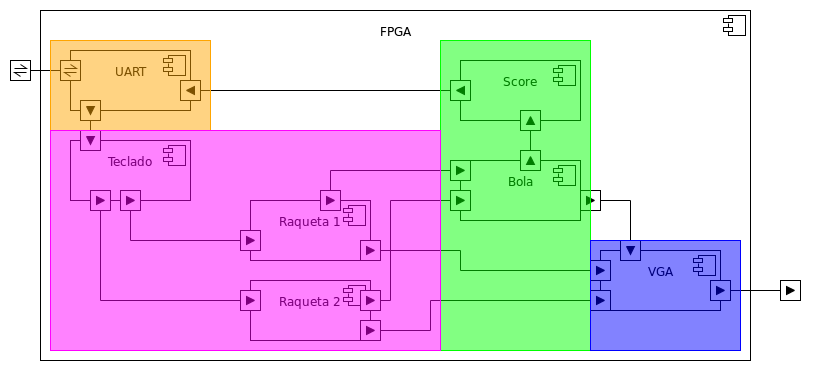
\includegraphics[width=1.0\textwidth]{images/fpga_componentes_timing.png}
  \caption{Distintos relojes utilizados.}
  \label{s3:fig:componentes-fpga-clocking}
\end{subfigure}
\caption{Diagrama de componentes implementados en la FPGA. }
\label{s3:fig:componentes-fpga-a}
\end{figure}


\subsubsection{Gestión de los relojes}
\label{s3:subsubsec:clocking}

\todo{Escribir, haciendo referencia a la
  figura~\ref{s3:fig:componentes-fpga-clocking}}

\subsection{Maletines ARM}
\label{s3:subsec:maletines}
\todo{Escribir esto, haciendo referencia a~\ref{s3:fig:FSM_maletin}. Si se
  decide mover la imagen a~\ref{s2:subsec:sistema-entero}, inventarse que
  poner. }\\
\todo{Sería interesante explicar lo del tecldo, y lo que se  hace para
  poder conectar varios maletines en serie.}

\begin{figure}[h]
  \centering
  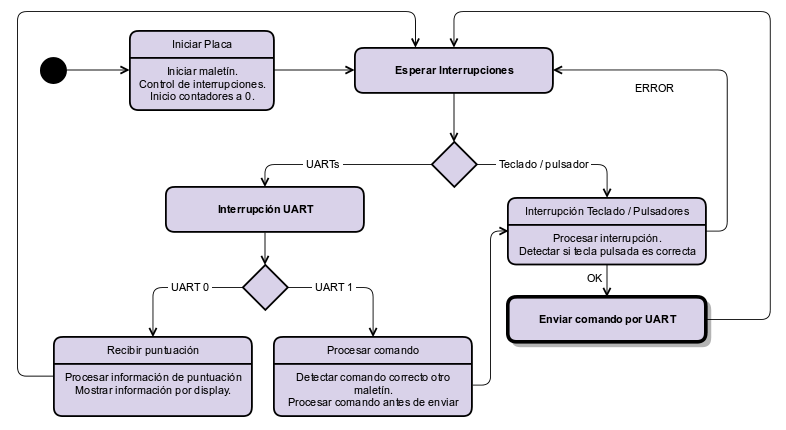
\includegraphics[width=1.0\textwidth]{images/maletin_fsm.png}
  \caption{FSM describiendo el comportamiento de los maletines.}
  \label{s3:fig:FSM_maletin}
\end{figure}





%
%
%%%
%%% Local Variables:
%%% mode: latex
%%% TeX-master: "../main.tex"
%%% End:


